%==============================================================================
% Sjabloon poster bachproef
%==============================================================================
% Gebaseerd op document class `a0poster' door Gerlinde Kettl en Matthias Weiser
% Aangepast voor gebruik aan HOGENT door Jens Buysse en Bert Van Vreckem

\documentclass[a0,portrait]{hogent-poster}

\usepackage{colortbl}
\usepackage{array}
\usepackage{float}

% Info over de opleiding
\course{Bachelorproef}
\studyprogramme{toegepaste informatica}
\academicyear{2024-2025}
\institution{Hogeschool Gent, Valentin Vaerwyckweg 1, 9000 Gent}

% Info over de bachelorproef
\title{Hoe kan een Secure Access Service Edge (SASE) architectuur geïmplementeerd worden binnen de hybride cloudomgeving van een software agency bedrijf}
%\subtitle{Ondertitel (eventueel)}
\author{Charan Chander}
\email{charan.chander@student.hogent.be}
\supervisor{dr. Pieter-Jan Maenhaut}
\cosupervisor{dhr. Louis De Jaeger}

% Indien ingevuld, wordt deze informatie toegevoegd aan het einde van de
% abstract. Zet in commentaar als je dit niet wilt.
\specialisation{Systeem- en Netwerkbeheer}
\keywords{SASE, Netskope, Hybride Cloud, Perimeterbeveiliging, Zero Trust}
\projectrepo{https://github.com/CharanChander/bachelorproef}

\begin{document}

\maketitle

%samenvatting
\begin{abstract}
  Het onderzochte softwarebedrijf kampt met toenemende uitdagingen op het gebied van netwerktoegang en beveiliging in zijn hybride cloud infrastructuur. De huidige perimetergebaseerde beveiliging biedt onvoldoende flexibiliteit en bescherming voor de moderne verspreide werkomgeving. Het ontwikkelde proof of concept implementeert een volledige Netskope SASE-architectuur met vijf kerncomponenten: Netskope Client, Next Gen Secure Web Gateway, Cloud Access Security Broker, Zero Trust Network Access en Netskope Publisher. De resultaten tonen aan dat de SASE-architectuur een effectieve oplossing biedt voor moderne beveiligingsuitdagingen.
\end{abstract}

\begin{multicols}{2} % This is how many columns your poster will be broken into, a portrait poster is generally split into 2 columns

\section{Probleemstelling}
Het onderzochte softwarebedrijf kampt met specifieke uitdagingen:

\begin{itemize}
\item Onvoldoende flexibiliteit van traditionele VPN-oplossingen voor remote werknemers
\item Beperkte zichtbaarheid en controle over cloud applicaties
\item Toenemende cybersecurity risico's door verspreide werkplek
\item Nood aan schaalbare beveiligingsoplossing die groeiambities ondersteunt
\end{itemize}

\vspace{1ex}

De centrale onderzoeksvraag luidt: 

\vspace{1ex}

\textbf{Hoe kan een SASE-architectuur worden geïmplementeerd binnen de hybride cloudomgeving van een softwarebedrijf gebruikmakend van het Netskope platform?}

\section{Methodologie}

Het onderzoek volgt een systematische vierfasenaanpak die zich uitstrekt over veertien weken:
\begin{center}
\renewcommand{\arraystretch}{1.7}
\begin{tabular}{|c|p{26cm}|c|}
\hline
\rowcolor{gray!20}
\textbf{Fase} & \textbf{Activiteit} & \textbf{Periode} \\
\hline
\rowcolor{blue!15}
\textbf{1} & \textbf{Literatuuronderzoek}, Bestudering, Analyse & Week 1-4 \\
\hline
\rowcolor{green!15}
\textbf{2} & \textbf{Requirements analyse}, Interviews, Evaluatie & Week 5 \\
\hline
\rowcolor{orange!15}
\textbf{3} & \textbf{Proof of Concept ontwikkeling}, Implementatie, Integratie & Week 6-12 \\
\hline
\rowcolor{red!15}
\textbf{4} & \textbf{Validatie \& evaluatie}, Testing, Feedback & Week 13-14 \\
\hline
\end{tabular}
\end{center}

\vspace{1ex}

\section{Resultaten}
Het ontwikkelde proof of concept toont concrete en meetbare resultaten:
\begin{center}
\renewcommand{\arraystretch}{1.7}
\begin{tabular}{|c|p{20cm}|c|}
\hline
\rowcolor{gray!20}
\textbf{Metric} & \textbf{Beschrijving} & \textbf{Resultaat} \\
\hline
\rowcolor{blue!15}
Apparatenfleet & Totaal beheerde apparaten & 122 apparaten \\
\hline
\rowcolor{purple!15}
Gebruikers & Actieve gebruikers in systeem & 121 gebruikers \\
\hline
\rowcolor{gray!20}
\textbf{Beveiliging} & \textbf{Beschrijving} & \textbf{Resultaat} \\
\hline
\rowcolor{green!15}
Malware Detection & Gedetecteerde malware instanties & 0 \\
\hline
\rowcolor{red!15}
Malicious Sites & Geblokkeerde kwaadaardige websites & 3 sites \\
\hline
\rowcolor{orange!15}
DLP Violations & Data Loss Prevention overtredingen & 2 gebruikers \\
\hline
\end{tabular}
\end{center}

\begin{center}
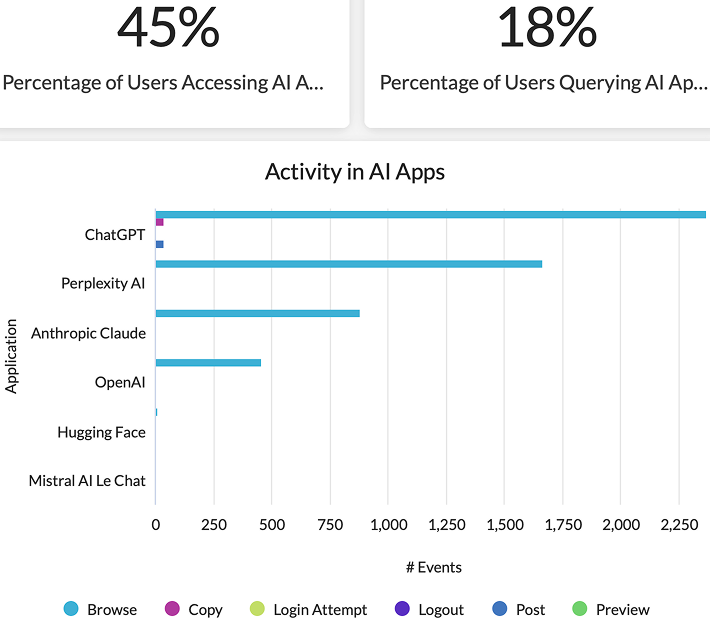
\includegraphics[width=0.9\columnwidth]{../graphics/AI-usage.png}\\
\textbf{Figuur:} AI Usage Policies Dashboard
\end{center}
Het Netskope platform toont significante AI-adoptie binnen de organisatie met 45\% van de gebruikers die toegang hebben tot AI-applicaties en 18\% die actief queries uitvoert. De platform-verdeling demonstreert een duidelijke voorkeur voor ChatGPT als dominante AI-tool, gevolgd door Perplexity AI en Anthropic Claude. Dit is waardevolle Business Intelligence voor het bedrijf, het biedt inzicht in gebruikersgedrag en applicatiegebruik.

\section{Conclusie}
De SASE implementatie via Netskope bewijst een praktisch haalbare en effectieve oplossing voor moderne hybride cloudomgevingen.

\textbf{Kernresultaten:}
\begin{itemize}
\item \textbf{Verbeterde beveiliging:} Zero Trust implementatie biedt contextbewuste beveiliging ongeacht locatie of apparaattype
\item \textbf{Operationele efficiëntie:} Geautomatiseerde policy management vermindert administratieve overhead aanzienlijk
\item \textbf{Schaalbaarheid:} Platform ondersteunt groeiambities en moderne werkpraktijken van software agencies
\item \textbf{Business Intelligence:} Advanced Analytics genereert waardevolle inzichten over applicatiegebruik en AI-governance
\end{itemize}

\textbf{Aanbevelingen voor vervolgonderzoek:}
\begin{itemize}
\item \textbf{Langetermijnanalyse:} Evaluatie van gebruikersadoptie over meerdere maanden
\item \textbf{ROI-analyse:} Kwantitatieve kostenbatenanalyse versus traditionele oplossingen
\end{itemize}
\end{multicols}
\end{document}